\chapter{Global optimization scheme} \label{ch:scheme}
In Chapter 1, it is introduced that optimizing the stiffness of the coupling robot in the manufacturing process can improve the manufacturing accuracy of the workpiece. The comparison and analysis of optimization methods through Chapter 2, the choice of using particle swarm optimization method to improve the stiffness of physically coupled robots in the manufacturing process. This chapter presents the development of a global optimization scheme for enhancing stiffness.
\section{Machining Process} \label{sec:scheme:process}
\subsection{Machining Path} \label{subsec:sec:scheme:process:path}
Machining is a process in which a material is cut to a desired final shape and size by a controlled material-removal process. The three principal machining processes are classified as turning, drilling and milling. The machining path is the path through space that the tip of a cutting tool follows to produce the desired geometry of the workpiece. The physically coupled robots perform coordinated machining tasks. Various machining tasks, such as drilling and milling, can be implemented if tools are attached to the coupler. 
\subsubsection{Path generation} \label{subsubsec:subsec:sec:scheme:process:path: path generation}
The given machining path is converted according to the G-code. G-code is the most widely used computer numerical control (CNC) programming language \cite{cncs}. It is used mainly in computer-aided manufacturing to control automated machine tools and has many variants. Extensions and variations of G-code have been added independently by control manufacturers and machine tool manufacturers, and operators of a specific controller must be aware of the differences between each manufacturer's product. In CNC machining centers, the G-code is composed of the letter G and two digits and is used for the control of tool paths, i.e., the movement of each feed axis, such as linear or arc interpolation, feed control, offset and transformation of the origin of the coordinate system, setting of dimensional units, tool offset and compensation. \par
The machining path can be generated using a combination of lines and arcs as the basic elements according to the G-code introduction above \cite{dqt}. Each element has a starting phase (velocity from zero to a constant value) and an ending phase (velocity from a constant value to zero). The basic elements overlap in their transition phases so that a line can be smoothly connected to an arc with a continuous position and velocity \cite{dqt}. \par
A $\boldsymbol{timeframes} = \left[t_{i,j}\right]_{n \times 4}$ can represent the relationship between a given machining path and time. $t_{i,1}$ represents the time value in the i-th element corresponding to a speed of 0 in the starting phase, $t_{i,2}$ represents the time value in the i-th element corresponding to a speed of a constant value in the starting phase, $t_{i,3}$ represents the time value in the i-th element corresponding to a speed of a constant value in the ending phase and $t_{i,4}$ represents the time value in the i-th element corresponding to a speed of 0 in the ending phase. $\boldsymbol{timeframes}$ can be shown as follows:
\begin{equation}
\boldsymbol{timeframes} = \begin{bmatrix} 
    t_{1,1} & \dots  & b_{1,4}\\
    \vdots & \ddots & \vdots\\
    b_{n,1} & \dots  & b_{n,4} 
    \end{bmatrix}
    \label{eq:tframe}
\end{equation}
According to the path characterization, there is a special relationship between $t_{i,3}$ and $t_{i+1,1}$ , $t_{i,4}$ and $t_{i+1,2}$. Then, based on the matrix (\ref{eq:tframe}), the following matrix $\boldsymbol{t}$ generated from the characteristic data can be obtained.
\begin{equation}
  \boldsymbol{t} =  \begin{bmatrix}
       t_{1,1} & \frac{t_{1,3}+t_{2,1}}{2} & \frac{t_{1,4}+t_{2,2}}{2} &  & \dots & \frac{t_{n-1,3}+t_{n,1}}{2} & \frac{t_{n-1,4}+t_{n,2}}{2} & t_{n,4} \end{bmatrix}
       \label{eq:t}
\end{equation}



\section{Data Pre-processing} \label{sec:Main:Pre-processing}
The challenge of enhancing stiffness is finding the stiffest configurations along the entire path, not at a single point. That means the coupled robot needs to move along a predefined machining path to ensure that the actual machining path matches the predefined path. The path is on the workpiece, and the workpiece can be placed freely in the space. In addition, evaluating and optimizing robots' configurations along a continuous machining path is time-consuming, so data pre-processing is needed to reduce the computation.


According to the path characterization, there is a special relationship between $t_{i,3}$ and $t_{i+1,1}$ , $t_{i,4}$ and $t_{i+1,2}$. Then, based on the matrix (\ref{eq:tframe}), the following matrix $\boldsymbol{t}$ generated from the characteristic data can be obtained.
\begin{equation}
  \boldsymbol{t} =  \begin{bmatrix}
       t_{1,1} & \frac{t_{1,3}+t_{2,1}}{2} & \frac{t_{1,4}+t_{2,2}}{2} &  & \dots & \frac{t_{n-1,3}+t_{n,1}}{2} & \frac{t_{n-1,4}+t_{n,2}}{2} & t_{n,4} \end{bmatrix}
       \label{eq:t}
\end{equation}
\subsection{Choice of sampling method}\label{subsec:sec:Main:Pre-processing:sampling method}
As the machining path is continuous and the stiffest configurataion of each point is very time-consuming and computationally intensive to evaluate, pre-processing of the data is required, and a sampling method can be used to extract sample points to reduce computation time. Commonly used sampling methods are equal distance sampling and equal time interval sampling. Since the previously listed sampling methods do not consider information on path point characteristics, such as information on straight and curved sections, they will increase the number of sampling points and thus the computational effort required to carry out the optimization process later. \par
In order to better take into account the feature information of the path points and to reduce the number of sampling points, resampling will be performed based on the above obtained time-dependent characteristic data matrix. \par
Firstly, intrroduce the resampling and its sampling process. The resampling is based on the data obtained from the previous matrix $\boldsymbol{data}$ relating to time, removing some unnecessary points to reduce the number of sampled points. \par
The resampling process is as follows:
\begin{itemize}
 \item \textbf{Step 1}: There is a series of points on the curve:$p_{0},p_{1}...p_{n-1},p_{n}$, as shown in
Figure \ref{fig:main:sampling1}.
\item \textbf{Step 2}: Calculate the distance of $p_{1},p_{2}...p_{n-1}$ to the line $p_{0},p_{n}$ as shown in
Figure \ref{fig:main:sampling2}.
\item \textbf{Step 3}: Find the maximum value of distance $p_{k}$, as shown in
Figure \ref{fig:main:sampling3}.
\item \textbf{Step 4}: If $p_{k}\leq d_\mathrm{tolerance}$, save $p_{0},p_{n}$ two points is sufficient. Else divide into two polylines at the point where $p_{k}$ is located and go to Step 2. $d_\mathrm{tolerance}$ is the required sampling tolerance.
\end{itemize}
\begin{figure}[h!]
\centering
\vspace{-1cm}
\setlength{\abovecaptionskip}{-1cm} 
\begin{minipage}[t]{0.48\textwidth}
\centering
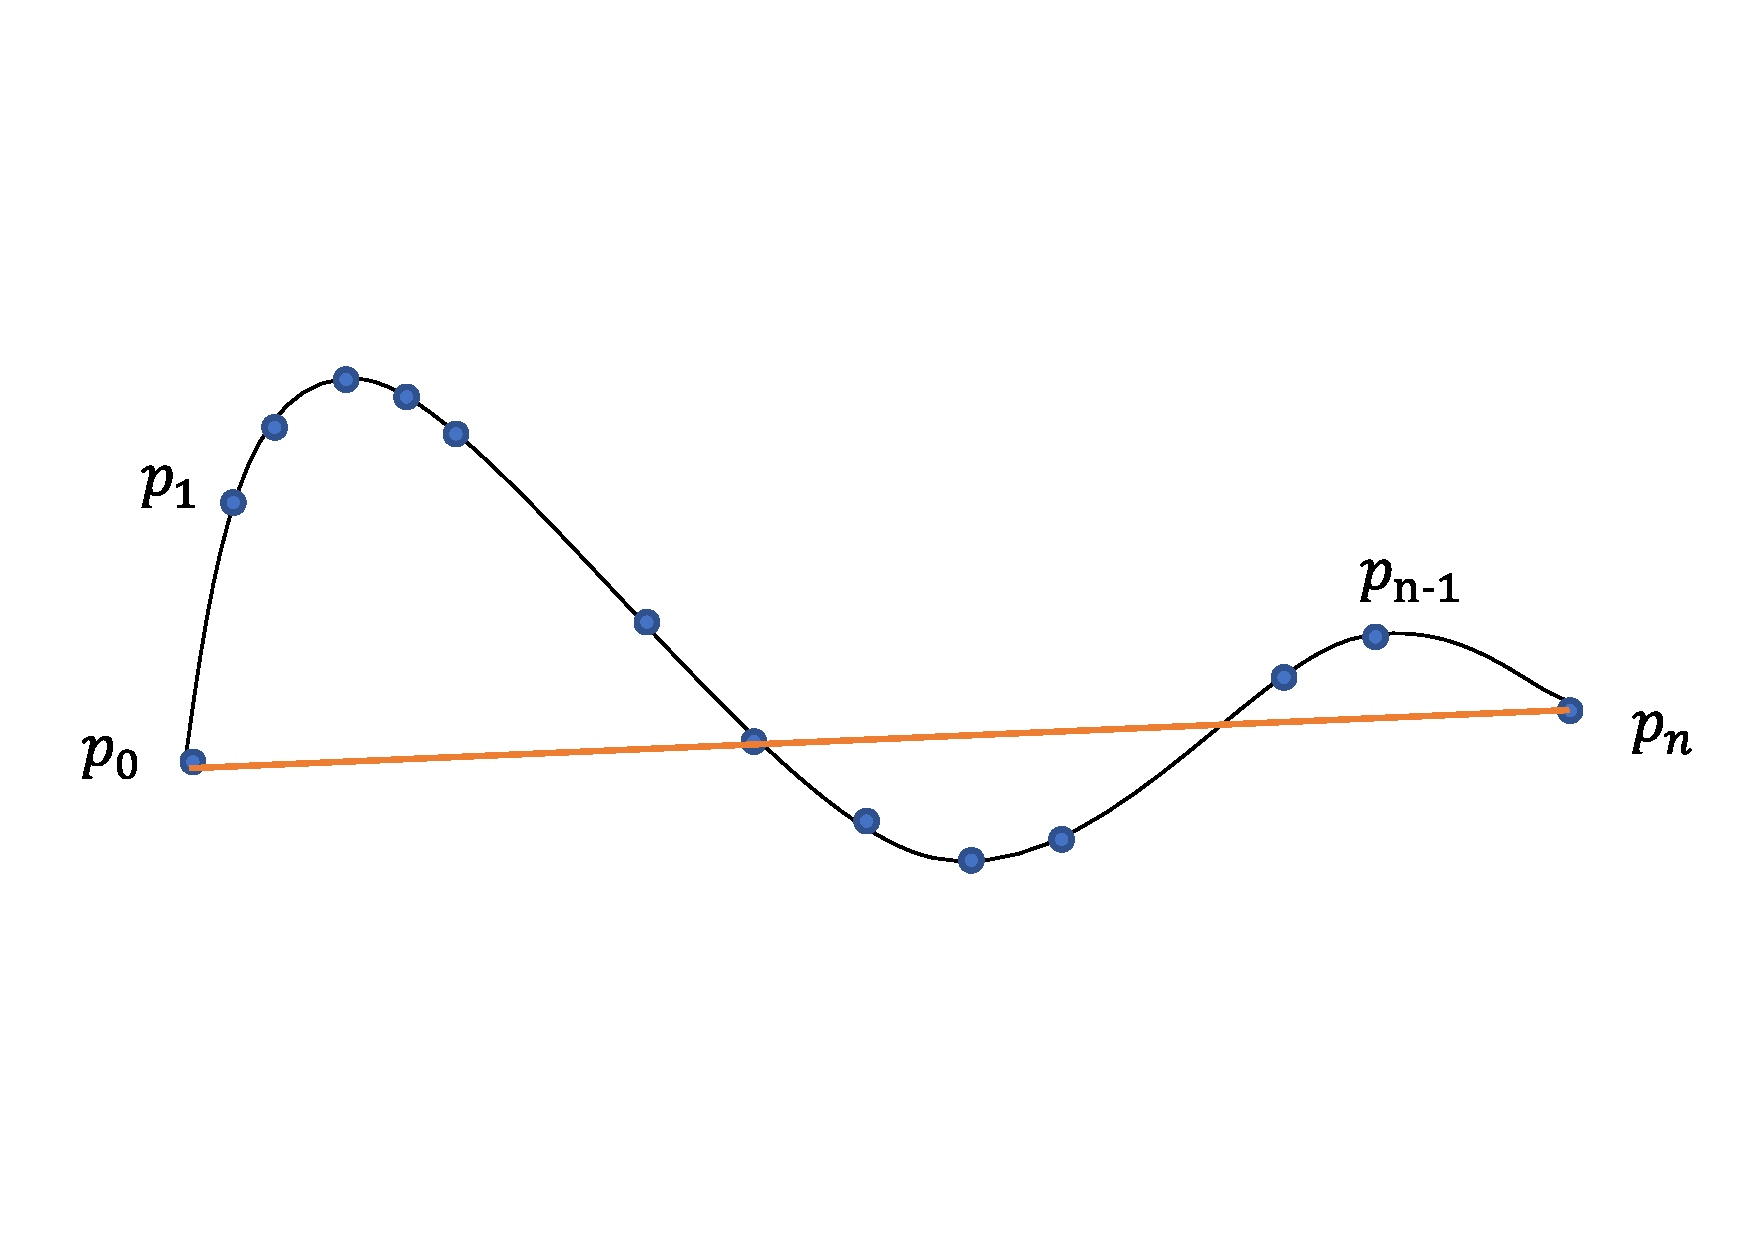
\includegraphics[width=6cm]{03_images/sampling_1.pdf}
\caption{Step 1}
\label{fig:main:sampling1}
\end{minipage}
\begin{minipage}[t]{0.48\textwidth}
\centering
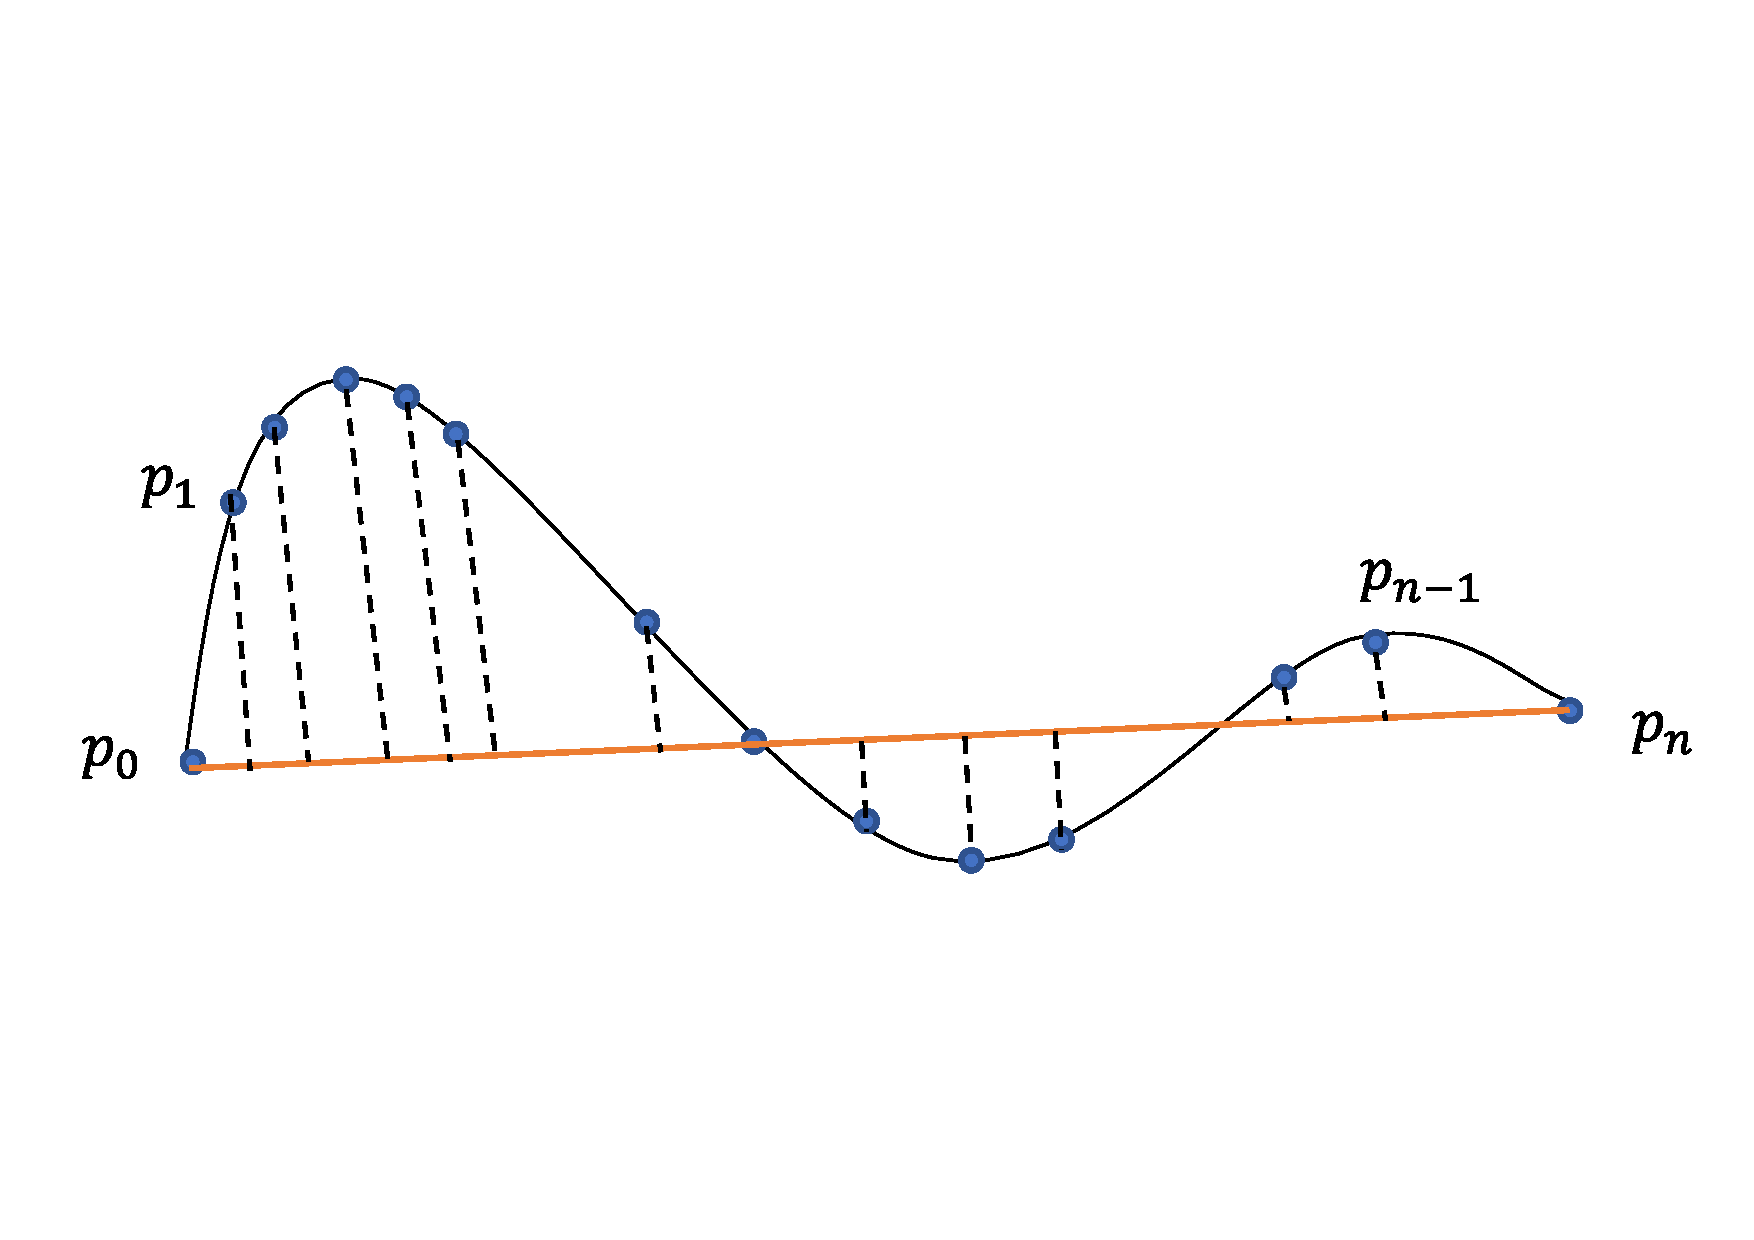
\includegraphics[width=6cm]{03_images/sampling_2.pdf}
\caption{Step 2}
\label{fig:main:sampling2}
\end{minipage}
\end{figure}
\begin{figure}[h!]
	\centering
        \vspace{-1.7cm}
        \setlength{\abovecaptionskip}{-1cm}
	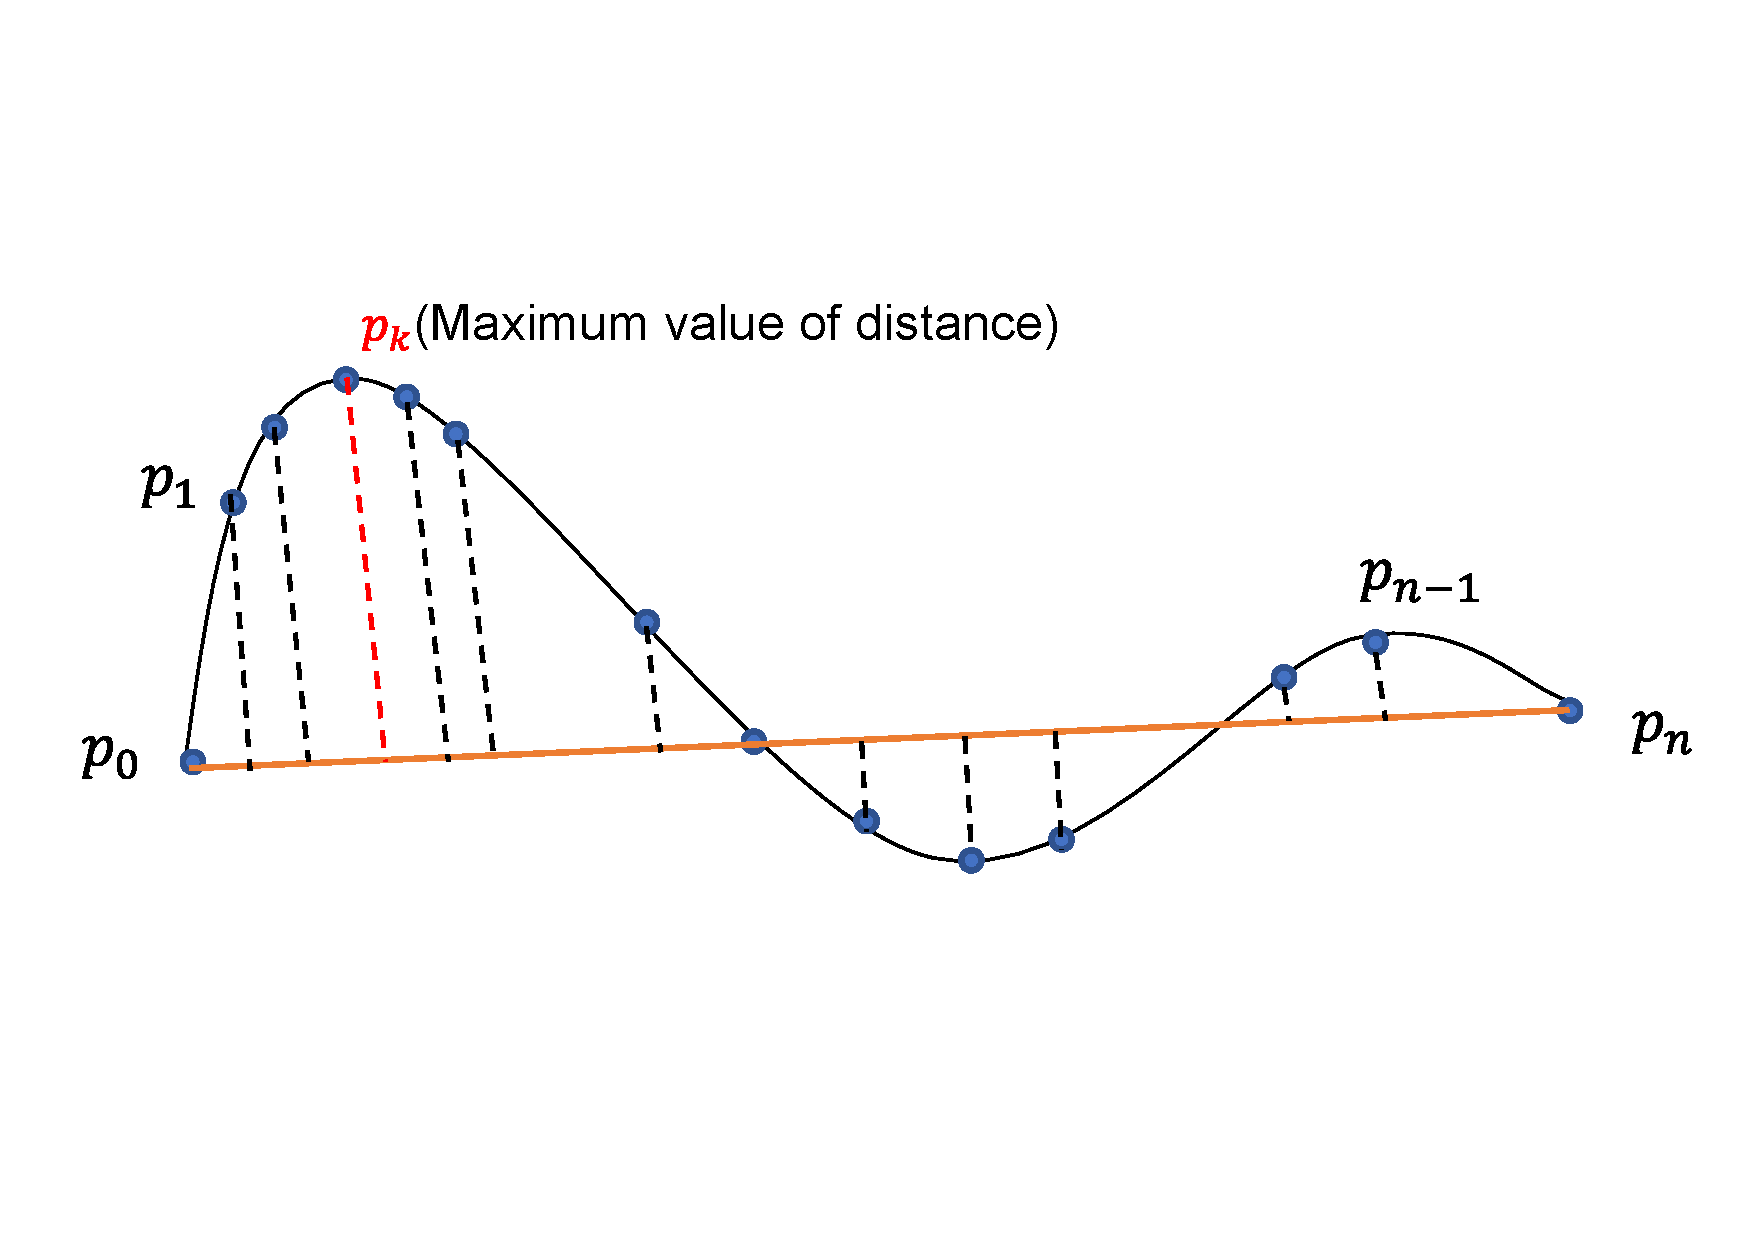
\includegraphics[width=6cm]{03_images/sampling_3.pdf}
	\caption{Step 3}
	\label{fig:main:sampling3}
\end{figure}
\subsection{Acquisition of sampled points for machining path }\label{subsec:sec:Main:Pre-processing:sampled points}
The resampling step was described in \ref{subsec:sec:Main:Pre-processing:sampling method}, and this section explains how to apply resampling to the data pre-processing process.\par
\begin{algorithm}
\SetAlgoLined
\caption{Resampling} \label{alg1} 
\KwData{ Maching path related data: $\boldsymbol{tframe},  \boldsymbol{data}$, Time corresponding to the start point of the currently analysed machining path: $t_\mathrm{start}$, Time corresponding to the end point of the currently analysed machining path: $t_\mathrm{end}$}
$t_{start}\gets \boldsymbol{data}(1)$\;
$t_{end}\gets \boldsymbol{data}(2)$\;
$\boldsymbol{sample_{traj}} \gets   \left[ \right]$\;
\While{$\boldsymbol{data} \neq \varnothing $}{
    \eIf{$\boldsymbol{data}$ contains only one element}{
    $ \boldsymbol{sample_{traj}} \gets \left[ \boldsymbol{data}(1) \right]$\; }
      {\If{$t_\mathrm{end} - t_\mathrm{start} > 0.01$}{
      Calculate the distance between the path points of equal time intervals to the corresponding points of $t_\mathrm{end}, t_\mathrm{start}$\;}
      {\eIf{$diff > dist$} 
        {Divide into two polylines at the point where $diff$ is located}
        {$\boldsymbol{sample_{traj}} \gets \begin{bmatrix}
       \boldsymbol{sample_{traj}} & t_{start} & t_{end}\end{bmatrix}$\;
        $\boldsymbol{data}(1)$ delete \;
        $t_{start}\gets \boldsymbol{data}(1)$\;
        $t_{end}\gets \boldsymbol{data}(2)$}}
        }
        }
\end{algorithm}
$ \boldsymbol{sample_{traj}}$: Matrix of the times corresponding to the sampled points after resampling, $diff$: The maximum value of distance, $dist$: The required limit value.\par
As shown in the Figure \ref{fig:main:samplepoints}, the shape after resampling can be seen as the same as the original curve, but the resampling only requires eleven sampling points.
\begin{figure}[h!]
	\centering
        \vspace{-3cm}
        \setlength{\abovecaptionskip}{-7.5cm}
	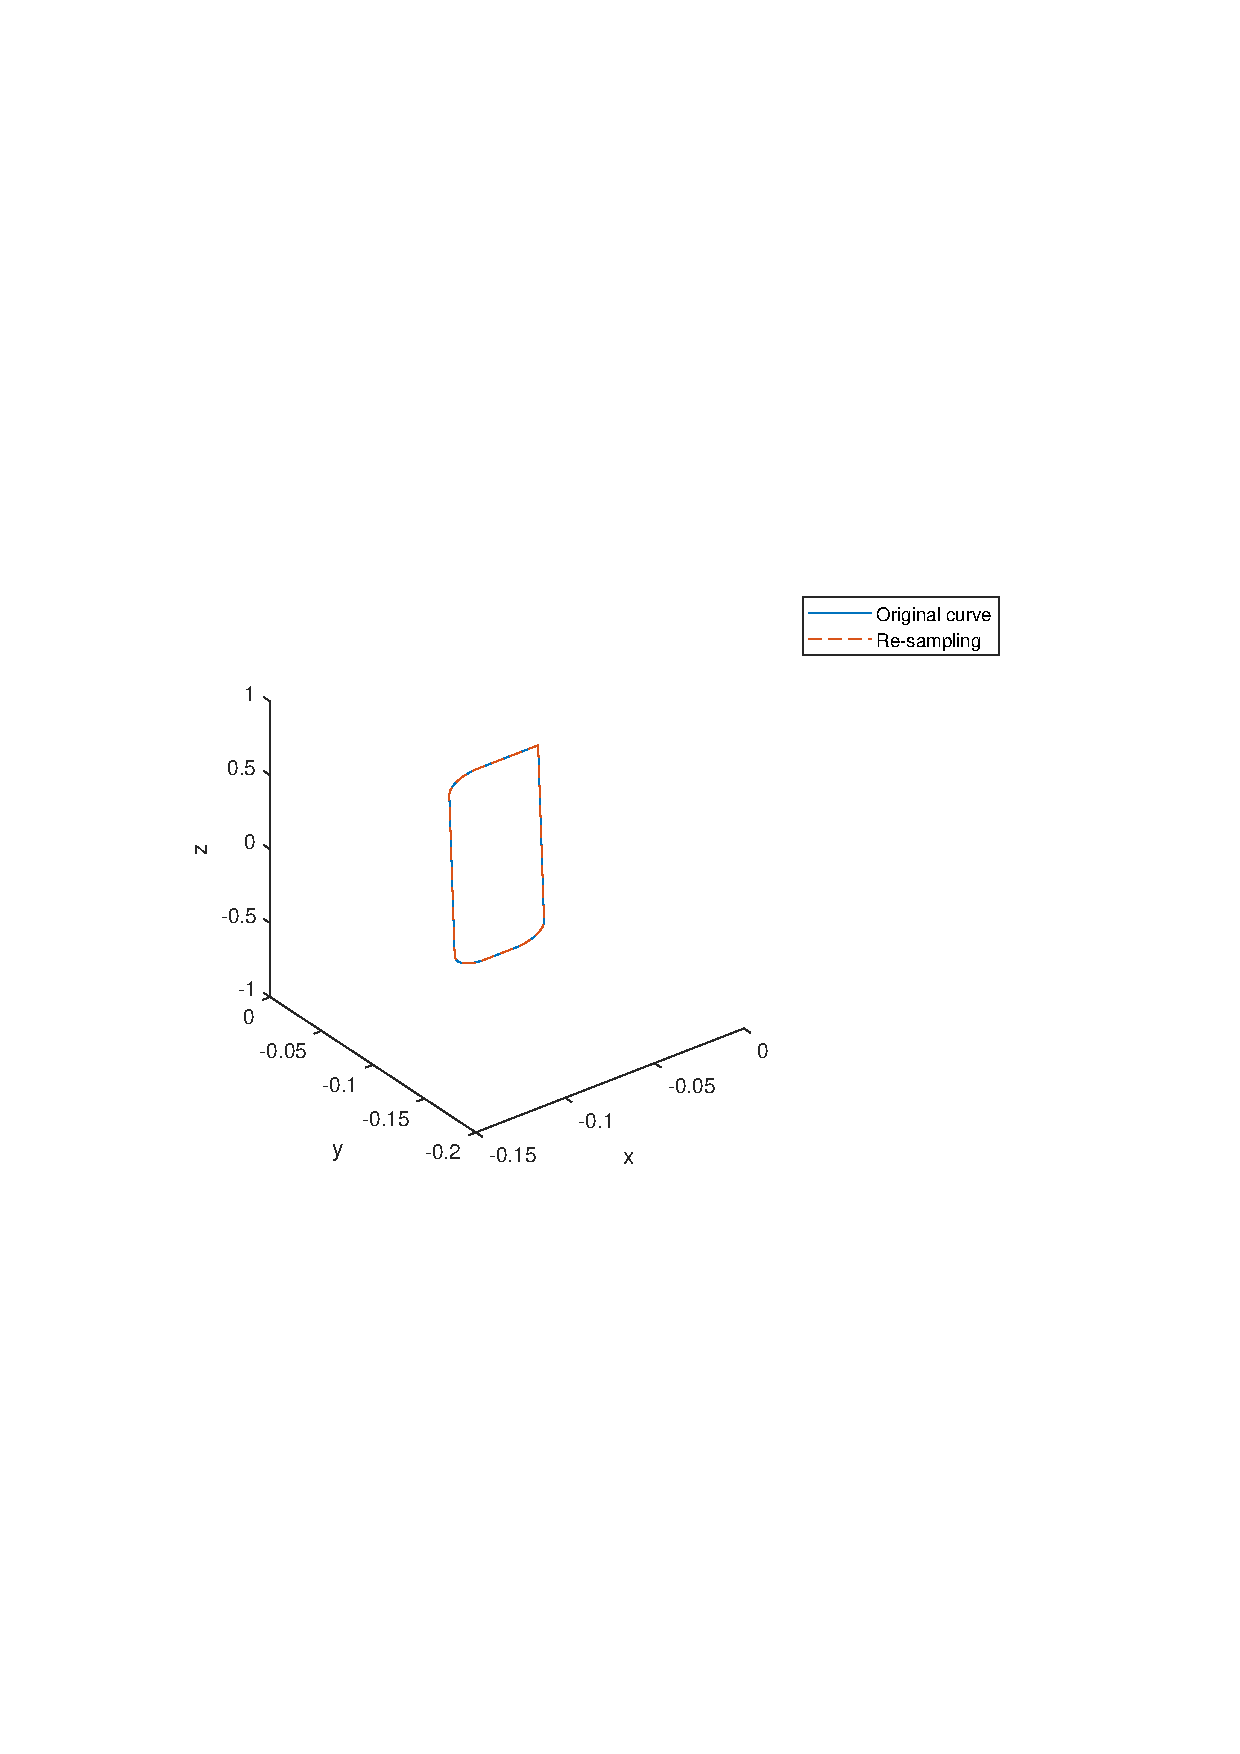
\includegraphics[width=\textwidth]{03_images/sample_point.pdf}
	\caption{Comparison of original and resampling curves}
	\label{fig:main:samplepoints}
\end{figure}
